\section{Softwarearchitektur}

\subsection{Strategie}


\subsection{Erkundung der Karte} \label{erkundungDerKarte}

\subsubsection{Kreisförmige Karte} ~\\

Hier geht es darum, dass die Karte keinen Rand hat. \\
Kurz beschreiben, dass wir zu Beginn eine begrenzte Karte hatten und dann eine offene Karte

\subsection{Entscheidungsverhalten der Agenten}

\subsubsection{Rollen} ~\\
Die Rollen werden in der Serverkonfiguration vorgegeben. In den Turnieren standen fünf Rollen bereit: default, worker, constructor, explorer und digger. \\
Die Rollen haben verschiedene Aktionen, welche sie ausführen dürfen. Zu Beginn haben alle Agenten die \textit{default}-Rolle inne. Diese enthält alle Standardaktionen wie \textit{move, rotate, skip, adopt, detach und clear}. Um nach verschiedenen Dingen suchen zu können, benötigen die Agenten die Rolle \textit{explorer}. Mit diesen kann ein \textit{survey} nach einem Dispenser gemacht werden. Sobald die Agenten die Aufgabe bekommen einen Block abzuholen, müssen sie in die Rolle \textit{worker} wechseln. Damit können sie Blocke aufnehmen, sich mit anderen Agenten verbinden und auch die Aufgaben abgeben. 
Die Besonderheit ist, dass alle Rollen die Aktionen der default-Rolle erben. Die Standardaktionen besitzen somit alle anderen Rollen ebenfalls.

Die Rolle \textit{constructor} und \textit{digger} hat die Gruppe nicht weiter verfolgt, da diese für unsere Strategie nicht notwendig war. 

\subsubsection{Aufgaben} ~\\
Um Punkte zu erzielen müssen Agenten verschiedene Aufgaben lösen. Der Server teilt den Agenten mit, wenn neue Aufgaben hinzukommen. Die Agenten müssen Blöcke bei den Dispensern abholen und in die Goalzones bringen. Damit eine Aufgabe abgegeben werden kann, müssen die Agenten die Blöcke in einer bestimmten Position angeordnet sein. Es gab Aufgaben mit einem, zwei, drei und vier Blöcken. Ab einem fixen Schritt im Spiel oder nach einer gewissen Anzahl an Abgaben, akzeptiert der Server eine Abgabe nicht mehr. Die Abgabefrist wird den Agenten bei der Bekanntmachung einer Aufgabe mitgeteilt. Über das Erreichen des Abgabelimits bekommen die Agenten allerdings keine Information.

Zu Beginn des Praktikums, wurde die Klasse \emph{NextTaskPlanner} implementiert. Da sich die Praktikumsgruppe dazu entschieden hat, dass in den ersten Turnieren nur Aufgaben mit einem Block auftreten, sollten unsere Agenten die Aufgabenplanung nicht absprechen, sondern die individuell beste Lösung finden. \emph{NextTaskPlanner} hat neue Aufgaben entgegen genommen und für alle Aufgaben Pläne erstellt.
Die Pläne wurden als Baumstruktur angelegt. Die Wurzel des Baumes war die Klasse \emph{NextPlanSolveTask}. Die Zweige des Baumes waren dann jeweilige Unterpläne, repräsentiert durch verschiedene Klassen für verschiene Teilaufgaben. Die Blätter des Baumes repräsentieren die auszuführenden Teilaufgaben für einen Agenten. Durch eine \emph{pre-order}-Suche wird die aktuell zu erfüllende Teilaufgabe gesucht. Jeden Schritt wird durch die Wurzel des Baumes geprüft, welche Teilaufgaben bereits erledigt sin. Diese werden dann durch die Suche nicht mehr zurück gegeben.
Jeder Plan berechnet, wie viele Schritte für die Erfüllung einer Aufgabe notwendig sind. \epmh{NextTaskPlanner} wählt dann den Plan aus, der die meisten Punkte in Relation zu den benötigten Schritten verspricht und lässt sich dann die jeweilige Teilaufgabe ausgeben um diese dem Agenten zu übergeben.
Falls eine Aufgabe nicht erfüllt werden kann, weil entweder keine Goalzone bekannt ist, oder die benötigten Dispenser fehlen, erzeugt \emph{NextPlanSolveTask} die benötigten Unterpläne, um die jeweiligen Sachen auf der Karte zu finden und löscht diese Unterpläne wieder, wenn dem Agenten alle Orte bekannt sind.

Bei späteren Turnieren wurden Aufgaben freigeschaltet, bei denen mehrere Blöcke abgegeben werden konnten. Da sich bei uns die Agenten zu einer Gruppe zusammenschließen, hat die Gruppe die weitere Planung der Aufgaben übernommen. Die Klasse \emph{NextTaskPlanner} wurde in die Gruppe ausgelagert. Der Agent war allerdings weiterhin für die Auswahl der Teilpläne zuständig. Die vorherigen Aufgaben des \emph{NextTaskPlanner} übernahm die Klasse \emph{NextTaskHandler}. 

Wenn eine Aufgabe das Ziel hatte zwei Blöcke abzugeben, dann wurden zwei Agenten ausgewählt um diese Aufgabe zu erfüllen. Die Klasse \emph{NextTaskPlanner} in der Gruppe teilte die Agenten den Aufgaben zu. Dabei wurde die Anzahl der Schritte pro verdientem Punkt minimiert und gleichzeitig verhindert, dass zu oft die gleiche Aufgabe Agentenpaaren zugeordnet wurde, damit die Agenten sich auf verschiedene Dispensertypen verteilen. Die Klasse \emph{NextTaskPlanner} bestimmte auch, welcher Agent zu welchen Dispenser läuft. Dazu wurden die Agenten gefragt, wie viele Schritte benötigt werden um zu einem Dispenser zu laufen und die  effizienteste Aufteilung gewählt.

Es kann ebenfalls vorkommen, dass Aufgaben mit einem Block effizienter waren oder es eine ungrade Anzahl an Agenten in einer Gruppe gab. In diesem Fall wurden den Agenten Aufgaben mit einem Block zugeordnet.

Die Entscheidung, welche Teilaufgabe zum aktuellen Zeitpunkt erfüllt werden muss, wurde durch dann durch die Klasse \emph{NextTaskHandler} berechnet. Dies geschah wiederum durch die oben beschriebene Baumstruktur. \\

\begin{tabular}{l | p{6cm}}\label{Liste der Pläne}
Klasse & Teilaufgabne \\
\hline
NextPlanExploreMap & Erkundung der Karte\\
NextPlanDispenser & Gang zu einem bestimmten Dispenser\\
NextPlanGoalzone & Gang in die nächste Goalzone\\
NextPlanRolezone & Gang in die nächste Rolezone\\
NextPlanSolveTask & Wurzel des Baumes\\
NextPlanSurveyDispenser & Suche nach nächstem bestimmten Dispenser\\
NextPlanSurveyGoalZone & Suche nach nächster Goalzone\\
NextPlanSurveyRoleZone & Suche nach nächster Rolezone\\
NextPlanSurveyRandom & Zufällige Schritte um Karte zu Beginn zu erkunden\\
NextPlanConnectToAgent & Verbindung zu einem anderen Agenten aufbauen\\
NextPlanDiscoverMapSize & Kartengröße bestimmen\\
NextPlanCleanMap & Goalzone und angrenzende Bereiche von Hindernissen befreien\\
\end{tabular}

\subsubsection{Wegfindung} \label{kap:wegfindung} ~\\
Random \newline
Spirale \newline
Manhattan \newline
A*

\subsubsection{Gruppenbildung} \label{kap:Gruppenbildung} ~\\

Gruppenbildung

\subsection{Globale und lokale Sicht}
Die Sicht der Agenten können in eine globale und eine lokalen Sicht unterschieden werden. Die globale Sicht besteht aus einer gespeicherten Karte pro Agent, die sich durch die Bewegungen des Agenten auf der Karte erweitert. Hier werden die verschiedenen Dinge wie Dispenser, Blöcke oder Zonen gespeichert. Sobald sich die Agenten in Gruppen finden, werden die Karten synchronisiert. Eine genauere Erklärung zu den Karten befindet sich im Kapitel \textit{\ref{erkundungDerKarte}}.\\

Die lokale Sicht des Agenten ist auf eine festgelegte Größe beschränkt. Die Sichtweite des Agenten wird in der Serverkonfiguration festgelegt. Bei einer Sichtweite von 5 sieht der Agent 5 Kästchen nach links, rechts, oben und unten, wie in Abbildung \ref{fig:agentensicht} dargestellt.
\begin{figure}
	\centering
	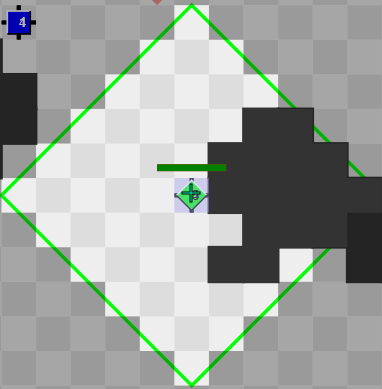
\includegraphics[width=150px]{bilder/agentensicht}
	\caption{Sicht des Agenten}
	\label{fig:agentensicht}
\end{figure}

Im ersten Schritt ermittelt der Agent einen möglichen Weg, wie er zu seinem Ziel gelangt. Hierfür wird der entsprechende Wegalgorithmus verwendet, welcher in Kapitel \textit{\ref{kap:wegfindung}]} genauer erläutert wird. Sobald der Weg ermittelt wurde und bevor ein Schritt des Weges beschritten wird, prüft der Agent auf Aktionen, welche vorher ausgeführt werden müssen. Diese Aktionen können einen Rollenwechseln beinhalten, ungenutzte Blöcke fallen lassen, einen Block vom Dispenser anfordern oder einen Block aufnehmen, eine Aufgabe in der Endzone abgeben oder sich mit einem anderen Agenten verbinden. Diese Aktionen sind Momentaufnahmen, die der Agent ausführen muss, bevor er zu einem neuen Ziel geht. Wenn keine dieser Aktionen passt, wird der Agent den Weg zu seinem Ziel gehen. Hier kommt nochmals eine Entscheidungsmöglichkeit für den Agenten in Frage. Ist der nächste Schritt frei und ich kann den Weg gehen, dann geht er diesen. Sollte aber beispielsweise ein Block in der Richtung sein, in die der Agent gehen möchte, so muss er diesen zunächst zerstören. Wenn ein Agent in der Richtung steht, so wird ein Weg um diesen Agenten herum erstellt. In Abbildung \ref{fig:agentensicht} wäre der Weg in Richtung Westen durch einen Block gehindert, sodass er diesen zunächst zerstören muss, bevor er in diese Richtung gehen kann. 

Zusammengefasst muss der Agent in jedem Schritt entscheiden, ob es eine Aktion gibt, die gerade notwendig ist, wie einen Block aufzunehmen oder ob der Schritt, den er gehen möchte, möglich ist.  

\subsection{Synchronisation und Kommunikation}
Die Kommunikation der Agenten funktioniert, sobald sie sich in einer Gruppe befinden. Die Synchronisation der Gruppen ist in Kapitel \textit{\ref{kap:Gruppenbildung}} genauer beschrieben. Für die Kommunikation wurde eine Schnittstelle entwickelt, welche die Nachricht, den Senderagenten und den Empfängeragenten in einer Nachrichtenbox bereithält. Stehen zwei Agenten um einen Dispenser und beide möchten einen Block anfordern, so wird der Agent zunächst prüfen, ob eine Nachricht für ihn vorliegt. Ist dies nicht der Fall, untersucht der Agent, ob andere Agenten in der nähe des Dispensers stehen. Wenn die Prüfung erfolgreich ist, so wird er eine Nachricht an den Agenten senden und dieser wird dann warten, bis der Dispenser frei ist. Er selbst stellt eine Anfrage an den Dispenser und nimmt den Block dann auf. 